\section{Definition of \textsc{TreeSketch}}
\label{apdx:ahle-sketch}

For simplicity, we shall define \textsc{TreeSketch} \citep{ahle2020oblivious} for inputs which are $r$-fold tensor products $x^{(1)}\otimes\dots\otimes x^{(r)}$ where $r$ is a power of two, and each $x^{(i)}\in\R^d$ is of the same dimension $d$.

The main ingredients will be two \emph{base} sketches, one for the leaves of the tree, and one for internal nodes. The leaf sketch, $T_\text{base}$ is a random matrix in $\R^{m\times d}$. The internal sketch, $S_\text{base}$, is a random matrix in $\R^{m\times m^2}$, which can be rapidly applied to the tensor product of two vectors in $\R^m$. It is possible to instantiate \text{TreeSketch} using simple sketches such as \textsc{CountSketch}, for the leaves, and \textsc{TensorSketch} for internal nodes. However, our theory we assumes that $T_\text{base}$ is \textsc{OSNAP} \citep{nelson2013osnap}, and $S_\text{base}$ is \textsc{TensorSHRT}, both of which enjoy a useful spectral property. 

Having picked the base sketches, we can define for any power of two $q\ge 2$, a random map $Q^q: \R^{m^q} \to \R^m$ whose action on a tensor product $v^{(1)}\otimes \dots\otimes v^{(q)}$ with $v^{(i)}\in\R^m$ is given by the following recursion:
\eq{
Q^q = Q^{q/2}(S^q_1(v^{(1)}\otimes v^{(2)})\otimes S^q_2(v^{(3)}\otimes v^{(4)})\otimes \dots\otimes S^q_{q/2}(v^{(q-1)}\otimes v^{(q)})).
}
Here, the matrices $(S^i_j)$ are independent copies of $S_\text{base}$. The action of \textsc{TreeSketch} $\Pi^r$ on $x^{(1)}\otimes\dots\otimes x^{(r)}$ is then defined by
\eq{
\Pi^r(x^{(1)}\otimes\dots\otimes x^{(r)}) = Q^r(T_1(x^{(1)})\otimes\dots \otimes T_r(x^{(r)}))
}
where the matrices $(T_i)$ are independent copies of $T_\text{base}$. Figure \ref{fig:treesketch} gives a schematic view of the computational tree for a tensor product with $r=4$. 

Whilst the action of $\Pi^r$ was only defined for tensor products, this can be extended to arbitrary vectors in $\R^{d^q}$. \citet{ahle2020oblivious} prove that the resulting linear sketch has many desirable subspace embedding properties, some of which are used in the proof of Theorem \ref{error bound theorem}.

\begin{figure}[b]
\begin{center}
    \scalebox{0.9}{
\tikzset{every picture/.style={line width=0.75pt}} %

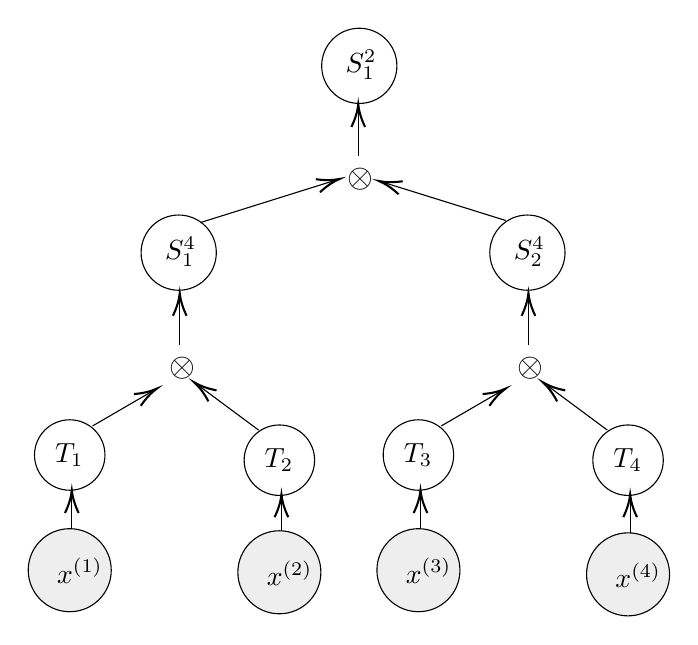
\begin{tikzpicture}[x=0.75pt,y=0.75pt,yscale=-1,xscale=1]

\draw    (148,113.5) -- (213.09,93.1) ;
\draw [shift={(215,92.5)}, rotate = 162.6] [color={rgb, 255:red, 0; green, 0; blue, 0 }  ][line width=0.75]    (10.93,-3.29) .. controls (6.95,-1.4) and (3.31,-0.3) .. (0,0) .. controls (3.31,0.3) and (6.95,1.4) .. (10.93,3.29)   ;
\draw    (295,112.5) -- (235.91,94.09) ;
\draw [shift={(234,93.5)}, rotate = 17.3] [color={rgb, 255:red, 0; green, 0; blue, 0 }  ][line width=0.75]    (10.93,-3.29) .. controls (6.95,-1.4) and (3.31,-0.3) .. (0,0) .. controls (3.31,0.3) and (6.95,1.4) .. (10.93,3.29)   ;
\draw    (176,213.5) -- (146.61,191.69) ;
\draw [shift={(145,190.5)}, rotate = 36.57] [color={rgb, 255:red, 0; green, 0; blue, 0 }  ][line width=0.75]    (10.93,-3.29) .. controls (6.95,-1.4) and (3.31,-0.3) .. (0,0) .. controls (3.31,0.3) and (6.95,1.4) .. (10.93,3.29)   ;
\draw    (96,211.5) -- (125.27,194.5) ;
\draw [shift={(127,193.5)}, rotate = 149.86] [color={rgb, 255:red, 0; green, 0; blue, 0 }  ][line width=0.75]    (10.93,-3.29) .. controls (6.95,-1.4) and (3.31,-0.3) .. (0,0) .. controls (3.31,0.3) and (6.95,1.4) .. (10.93,3.29)   ;
\draw    (138,172.5) -- (138,149.5) ;
\draw [shift={(138,147.5)}, rotate = 90] [color={rgb, 255:red, 0; green, 0; blue, 0 }  ][line width=0.75]    (10.93,-3.29) .. controls (6.95,-1.4) and (3.31,-0.3) .. (0,0) .. controls (3.31,0.3) and (6.95,1.4) .. (10.93,3.29)   ;
\draw    (86,264.5) -- (86,244.5) ;
\draw [shift={(86,242.5)}, rotate = 90] [color={rgb, 255:red, 0; green, 0; blue, 0 }  ][line width=0.75]    (10.93,-3.29) .. controls (6.95,-1.4) and (3.31,-0.3) .. (0,0) .. controls (3.31,0.3) and (6.95,1.4) .. (10.93,3.29)   ;
\draw    (187,266.5) -- (187,246.5) ;
\draw [shift={(187,244.5)}, rotate = 90] [color={rgb, 255:red, 0; green, 0; blue, 0 }  ][line width=0.75]    (10.93,-3.29) .. controls (6.95,-1.4) and (3.31,-0.3) .. (0,0) .. controls (3.31,0.3) and (6.95,1.4) .. (10.93,3.29)   ;
\draw    (344,213.5) -- (314.61,191.69) ;
\draw [shift={(313,190.5)}, rotate = 36.57] [color={rgb, 255:red, 0; green, 0; blue, 0 }  ][line width=0.75]    (10.93,-3.29) .. controls (6.95,-1.4) and (3.31,-0.3) .. (0,0) .. controls (3.31,0.3) and (6.95,1.4) .. (10.93,3.29)   ;
\draw    (264,211.5) -- (293.27,194.5) ;
\draw [shift={(295,193.5)}, rotate = 149.86] [color={rgb, 255:red, 0; green, 0; blue, 0 }  ][line width=0.75]    (10.93,-3.29) .. controls (6.95,-1.4) and (3.31,-0.3) .. (0,0) .. controls (3.31,0.3) and (6.95,1.4) .. (10.93,3.29)   ;
\draw    (306,172.5) -- (306,149.5) ;
\draw [shift={(306,147.5)}, rotate = 90] [color={rgb, 255:red, 0; green, 0; blue, 0 }  ][line width=0.75]    (10.93,-3.29) .. controls (6.95,-1.4) and (3.31,-0.3) .. (0,0) .. controls (3.31,0.3) and (6.95,1.4) .. (10.93,3.29)   ;
\draw    (254,264.5) -- (254,244.5) ;
\draw [shift={(254,242.5)}, rotate = 90] [color={rgb, 255:red, 0; green, 0; blue, 0 }  ][line width=0.75]    (10.93,-3.29) .. controls (6.95,-1.4) and (3.31,-0.3) .. (0,0) .. controls (3.31,0.3) and (6.95,1.4) .. (10.93,3.29)   ;
\draw    (355,266.5) -- (355,246.5) ;
\draw [shift={(355,244.5)}, rotate = 90] [color={rgb, 255:red, 0; green, 0; blue, 0 }  ][line width=0.75]    (10.93,-3.29) .. controls (6.95,-1.4) and (3.31,-0.3) .. (0,0) .. controls (3.31,0.3) and (6.95,1.4) .. (10.93,3.29)   ;
\draw    (224,81.5) -- (224,58.5) ;
\draw [shift={(224,56.5)}, rotate = 90] [color={rgb, 255:red, 0; green, 0; blue, 0 }  ][line width=0.75]    (10.93,-3.29) .. controls (6.95,-1.4) and (3.31,-0.3) .. (0,0) .. controls (3.31,0.3) and (6.95,1.4) .. (10.93,3.29)   ;

\draw    (137.5, 128) circle [x radius= 18.12, y radius= 18.12]   ;
\draw (128,117.4) node [anchor=north west][inner sep=2pt]    {$S_{1}^{4}$};
\draw    (224.5, 38) circle [x radius= 18.12, y radius= 18.12]   ;
\draw (215,27.4) node [anchor=north west][inner sep=2pt]    {$S_{1}^{2}$};
\draw    (186, 228) circle [x radius= 16.97, y radius= 16.97]   ;
\draw (176,219.4) node [anchor=north west][inner sep=2pt]    {$T_{2}$};
\draw (126,171.4) node [anchor=north west][inner sep=5pt]  [font=\large]  {$\otimes $};
\draw    (85, 225.5) circle [x radius= 16.97, y radius= 16.97]   ;
\draw (75,216.9) node [anchor=north west][inner sep=2pt]    {$T_{1}$};
\draw  [fill={rgb, 255:red, 238; green, 238; blue, 238 }  ,fill opacity=1 ]  (85, 281) circle [x radius= 20, y radius= 20]   ;
\draw (76,272.4) node [anchor=north west][inner sep=2pt]    {$x^{(1)}$};
\draw  [fill={rgb, 255:red, 238; green, 238; blue, 238 }  ,fill opacity=1 ]  (186, 282) circle [x radius= 20, y radius= 20]   ;
\draw (177,273.4) node [anchor=north west][inner sep=2pt]    {$x^{(2)}$};
\draw    (305.5, 128) circle [x radius= 18.12, y radius= 18.12]   ;
\draw (296,117.4) node [anchor=north west][inner sep=2pt]    {$S_{2}^{4}$};
\draw    (354, 228) circle [x radius= 16.97, y radius= 16.97]   ;
\draw (344,219.4) node [anchor=north west][inner sep=2pt]    {$T_{4}$};
\draw (294,171.4) node [anchor=north west][inner sep=5pt]  [font=\large]  {$\otimes $};
\draw    (253, 225.5) circle [x radius= 16.97, y radius= 16.97]   ;
\draw (243,216.9) node [anchor=north west][inner sep=2pt]    {$T_{3}$};
\draw  [fill={rgb, 255:red, 238; green, 238; blue, 238 }  ,fill opacity=1 ]  (253, 281) circle [x radius= 20, y radius= 20]   ;
\draw (244,272.4) node [anchor=north west][inner sep=2pt]    {$x^{(3)}$};
\draw  [fill={rgb, 255:red, 238; green, 238; blue, 238 }  ,fill opacity=1 ]  (354, 283) circle [x radius= 20, y radius= 20]   ;
\draw (345,274.4) node [anchor=north west][inner sep=2pt]    {$x^{(4)}$};
\draw (212,80.4) node [anchor=north west][inner sep=5pt]  [font=\large]  {$\otimes $};
\end{tikzpicture}
}
    \caption{Schematic view of the computational tree for \textsc{TreeSketch} for a tensor product of four vectors $x^{(1)}\otimes\dots\otimes x^{(4)}$.}
    \label{fig:treesketch}
\end{center}
\end{figure}